\documentclass[D:/studies/WinnerS/Erhebungen/IPhO1718/paper/problem_solving/main/TaylorFrancis/interactapasample]{subfiles}

\begin{document}

\section{Methodology}

In order to study the extent to which success in the Olympiad is a function of cognitive and motivational variables, we employ a statistical modelling approach. In line with the nomological-deductive paradigm \cite{Bortz.2002}, statistical models test statements about reality. In particular, statistical significance tests can be utilized as indicators for the relevance of statistical models. The included predictors in the models are gleaned from the expectancy-value model (such as expectancy and values towards the physics Olympiad) \citep{Eccles.1983,Urhahne.2012} and were developed based on other research where no viable measures were applicable. The reliability of the included measures need to be assessed in order to include meaningful variables in the statistical models. Furthermore, measures of reliability and validity can ensure that the models are meaningful.


\section{Assessing physics problem solving abilities}

A major developmental task was the implementation of problem solving measures applicable to high-achieving students in physics. \cite{Maloney.2011} suggests that the nature of the tasks in an investigation (well- versus ill-defined; quantitative versus qualitative), and the definition of what problem solving skills entail should be made explicit. Based on the literature review on physics expertise, a self-reported open-ended question was chosen as a measurement tool in order to assess students' reflective thinking about problem solving. The open-ended responses were coded using a theory-based coding rubric.

In order to develop a theory-based coding rubric, relevant research on physics problem solving was revisited. For example, \cite{Leonard.1996} propose a measure for physics problem solving that assesses the strategies that students use to solve problems. Strategies, as the authors use the term, entail the concept to solve the problem, a justification for why the concepts can be applied (i.e., conditional knowledge), and a procedure by which the concept is applied. The authors emphasize the role of conceptual knowledge that is important for physics problem solving and the idea that problem solving strategies shall be established before applying mathematics. 

A similar rationale was adopted in the current assessment for problem solving skills. I.e., students were asked to write down the physics ideas that they would use to solve the well-defined physics problem without going through the whole problem solution process (i.e., leaving out problem representation and mathematical routines). Consequently, the items provided the students space to construct their understanding and give context to their thoughts \citep{Hammann.2014}. In order to make clear to students what was meant with the prompt, an example was provided to all students that they read through. Afterwards, four physics problems (two mechanics, two electro-magnetism) followed that each had a certain context and well-defined solution plans.

The theory-based coding rubric utilized scoring categories that were implemented in prior research. \cite{Docktor.2016} developed a coding rubric for students' written solutions for physics problems. This rubric is also useful for the current study, however, not all of the five categories were adopted for our measure. Our coding rubric comprised the categories concept, execution, context, and detail. In the following, definitions of the categories are provided. We indicate in brackets what the corresponding categories from the study by \cite{Docktor.2016} are. Concept entails information if students provide all relevant concepts that are necessary for solving the problem (physics approach). Execution entails information about the comprehensiveness of the response (logical progression). Context reflects the assumptions and conditions for applying the concepts (specific application of physics) \citep{Fortus.2009}, and, finally, detail detected when students' interspersed their response with an elaboration of the concepts such as through mathematical formulas where the relevant variables became clear. Furthermore, these aspects also relate to the strategy definiton in \cite{Leonard.1996}. 

Similar to the rubric by \cite{Docktor.2016}, all categories were graded with $0$ to $2$ points. Moreover, concept and context could be graded negative ($-1$) when a concept was wrong (e.g., when students used magnetic force instead of electric force in a problem). For concept the full score was given when the student response included all concepts that were central to the respective problems. Execution pertained the presentation of the physical ideas. If the sentences were understandable (not only two-word phrases) and logically connected, full credit was given. Full credit for detail was awarded when all relevant variables in the concepts were identified. Full credit for context was given when important assumptions and boundary conditions were identified (e.g., frictionless slide). Note that the categories are not idependent of each other. As a consequence, we aggregated the score for each student to an overall measure which is henceforth called ability of problem conceptualization, because a full credit (i.e., $8$ points for each problem) would indicate that the student has all the relevant analyses correct that would count for successful physics problem solving.

Four physics problems were presented to the students that are related to two fundamental physics topics that are encountered throughout physics: mechanics and electro-magnetism. Knowledge for gravitational and electro-magnetic force, momentum, and energy conservation were necessary to solve all problems. 

\subsubsection*{Example}

\begin{tcolorbox}
A mass runs through a looping (see picture below). The mass starts from a heights above the highest point of the looping. The movement is frictionless.

Determine the minimal necessary heights for the mass, so that the mass can run through the looping without falling down. Assume that the mass does not slip and that it is a point mass.

\textit{Describe how you would solve this problem and what physics ideas you would use to solve it. Try to write full sentences.}

\begin{center}
\subfile{D:/studies/WinnerS/Erhebungen/IPhO1718/paper/problem_solving/method/img/sample_problem}
\end{center}
\end{tcolorbox}

In addition to the open ended item, the students were also given a test for conceptual knowledge that taxed more the declarative aspect of the knowledge that comes to bearing in solving these problems:

\begin{tcolorbox}

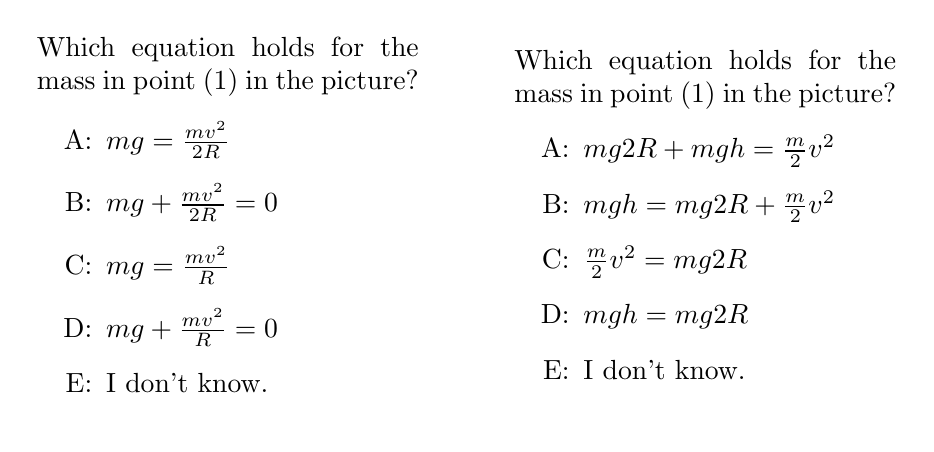
\begin{tikzpicture}

\node at (0,0) {\parbox{.4\linewidth}{Which equation holds for the mass in point (1) in the picture? 
\begin{itemize}
\item[A:] $ m g=\frac{m v^2}{2 R} $
\item[B:] $ mg + \frac{m v^2}{2 R}=0 $
\item[C:] $ mg = \frac{m v^2}{R} $
\item[D:] $ mg + \frac{m v^2}{R}=0 $
\item[E:] I don't know.
\end{itemize}}};

\node at (.5\linewidth,0) {\parbox{.4\linewidth}{Which equation holds for the mass in point (1) in the picture? 
\begin{itemize}
\item[A:] $ mg2R + mgh =\frac{m}{2} v^2 $
\item[B:] $ mgh = mg2R + \frac{m}{2} v^2 $
\item[C:] $ \frac{m}{2}v^2 = mg2R $
\item[D:] $ mgh = mg2R $
\item[E:] I don't know.
\end{itemize}}};

\end{tikzpicture}

\end{tcolorbox}

An expert answer for the open-ended problem looked as follows: 
\begin{quote}
The centrifugal force at the highest point of the looping needs to be equal with the weight: $(m*v^2)/r=m*g$. In order to figure out how high the starting point needs to be, we calculate the initial speed that he needs in order to pass the looping and with the energy conservation law we determine the height: $v=\text{sqrt}(g*r), \; mgh=m/2*v^2 h=0.5r+2r$ (height of the looping) $h=5/2R$.

% Die Fliehkraft muss am h\"o{}chsten Punkt des Looping, genau so gross [sic!] sein wie die Gewichtskraft: $(m*v^2)/r=m*g$. Um herauszufinden wie hoch der Startpunkt sein muss, berechnen wir zun\"a{}chst die Anfangsgeschwindigkeit die er braucht um das Looping zu schaffen und \"u{}ber den Energieerhaltungssatz daraus die H\"o{}he $h$: $v=\text{sqrt}(g*r), \; mgh=m/2*v^2 h=0.5r+2r$ (H\"o{}he Looping) $h=5/2R$.
\end{quote}

In this answer, $2$ points were given for the concepts (equilibrium of forces and energy conservation). Furthermore the student's answer is coherent and it is easy for the reader to follow ($2$ points for execution). Details are given through the correct formulas. Missing points appear for the context, because the student does not include a reflection of boundary conditions in the response. A novice response, were no credit is awarded, looked like this:
\begin{quote}
I would recognize the ascent of the trajectory and the height of the looping. Besides, I think the mass of the object is crucial. At first I would calculate the velocity or acceleration on the initial path and the velocity with which the object enters the looping. With the gravitational acceleration and the initial acceleration you could calculate which acceleration and initial height is necessary that the object does not fall out the looping.

%Ich würde die Steigung der Bahn und die Höhe des Loopings beachten. Außerdem ist meiner Meinung nach die Masse des Körpers entscheidend. Als erstes würde ich die Geschwindigkeit bzw. Beschleunigung auf der Startstrecke berechnen und die Geschwin\-digkeit, mit der der Körper in den Looping eintrifft. Aus der Gravitationsbeschleunigung und der Anfangsbeschleunigung könnte man ausrechnen, welche Beschleunigung und somit Anfangshöhe erforderlich ist, damit der Körper nicht aus dem Looping fällt.
\end{quote}

In order to validate the ratings, two raters (first author and physics undergraduate student with extensive experience in math and physics) that were familiarized with the problems coded the student responses. Both raters were trained to score the responses with regards to the rubric. All student responses were scored. When both raters disagreed, the disagreements were discussed and eventually a consensus was reached with regards to the final scoring.



\end{document}